\subsection{Numerical Investigation of Propagating Modes in TEM Cells}\label{sec:modes_tem_cell}
\subsubsection{Mathematical derivation}
% Goal is to describe the modes in a TEM cell, including their cut-off frequencies. \cite{Kreindl_Bauernfeind_Weiss_Stockreitner_Kaltenbacher_2024} shows that these investigations are important. There are also modes propagating perpendicular to the intended propagation direction. Why are no waveguides used? Explain.

% In this paper, a VCSEL with a decoupling capacitor are modeled. It is visible, that the electric coupling dominates at an orientation of 90°. A local minimum is then visible. At 400\,MHz and upwards, inductive coupling becomes dominant, but only at 0° where it couples with the septum. It is possible, that a certain mode can propagate at a certain frequency, which influenced the result in this paper. 


Any electromagnetic field distribution in a waveguide can be represented by an infinite series of normal modes. \autoref{eqn:norm_power} shows that each mode is orthogonal to each other, with $\mathbf{e_n}^\pm$ and $\mathbf{h_n^\pm}$ being the function vectors of the electric and magnetic field in transverse direction \cite{Collin_2015}. A coupling between the modes only occurs due to geometric changes of the waveguide. Additionally, each mode is normalized to $\sqrt{\mathrm{W}}$, shown by \autoref{eqn:unit_power}. Only the transverse fields are investigated in these Equations, because they carry power along the waveguide, opposed to the fields in the propagation direction.

\begin{align}
    \iint \mathbf{e_n^\pm}\times \mathbf{h_m^\pm}\mathrm{d}S\mathbf{n}&=0 \quad\text{if}\quad n\neq m
    \label{eqn:norm_power}\\
    \iint \mathbf{e_n^\pm}\times \mathbf{h_n^\pm}\mathrm{d}S\mathbf{n}&=1
    \label{eqn:unit_power}
\end{align}

The radiated fields can be described by a summation of normal modes, as in \autoref{eqn:modal_superposition1} and \autoref{eqn:modal_superposition2}. The coefficients of these modes are straightforward to calculate, due to Lorentz Reciprocity Theorem, if the waveguide's walls are perfectly conducting. Ideally, any higher order mode than the first TEM mode will be suppressed, and the calculation simplifies to $n=0$. Additionally, it is assumed that the source is electrically small, which makes it possible to represent it with dipoles, further simplifying the equations \cite{Koepke_1989}. 

\begin{align}
    \mathbf{E^\pm}&=\sum_na_n\mathbf{E_n^\pm}    \label{eqn:modal_superposition1}\\
    \mathbf{H^\pm}&=\sum_na_n\mathbf{H_n^\pm}    \label{eqn:modal_superposition2}
\end{align}

Suppose a current source $\mathbf{J_1}$ excites a waveguide (as is the case with the dipoles in the TEM cell). Normally, such a current source would be driven with external fields, but for the sake of the argument, they are ignored. Only $\mathbf{E}$ and $\mathbf{H}$ are considered, which are the fields radiated by $\mathbf{J_1}$. Additionally, $\mathbf{E}_n^\pm$ and $\mathbf{H}_n^\pm$ are the resulting waveguide fields, with the signs indicating the direction of propagation. Take \autoref{eqn:lorentz_rec_theorem_int} and set $\mathbf{J_2}=\mathbf{M_1}=\mathbf{M_2}=0$. Now, only the current source $\mathbf{J_1}$ remains, and the \autoref{eqn:J1_propagating_waves} emerges. % Explain how certain surfaces do not to have be integrated, therefore rendering this equation very useful. Also, the expansion coefficients can be determined. Maybe do this calculation with a rectangular waveguide.

\begin{equation}
    \oiint _S (\mathbf{E_n^\pm}\times \mathbf{H}-\mathbf{E}\times \mathbf{H}_n^\pm)\cdot\mathrm{d}\mathbf{S}=\iiint \mathbf{J_1}\cdot\mathbf{E_n^\pm}\mathrm{d}V
    \label{eqn:J1_propagating_waves}
\end{equation}

In case of the TEM cell, it is desirable that only the TEM mode is propagating, and that the source is represented by a dipole. Considering an electric dipole, therefore, the \autoref{eqn:dipole_tem_waves} arises. In this equation, the wave amplitudes $a$ and $b$ are given through the surface integral in the Lorentz Reciprocity theorem, with $a$ being the wave going to the left side, and $b$ to the other. The electric dipole moment $\mathbf{e_m}$ is given by the current $\mathbf{J}$ flowing through the infinitesimal wire. Note that only the electric field of TEM wave propagation is considered. In reality, more modes may propagate, for which the electric field must be replaced by the superposition of normal modes as in \autoref{eqn:modal_superposition1}. %Additionally, to calculate the exact value of the electric field, a series of image sources as a Green's function may be applied.

\begin{equation}
\begin{pmatrix}a \\b\end{pmatrix} = -\frac{1}{2}\mathbf{m_e}\cdot \mathbf{E}^\pm
\label{eqn:dipole_tem_waves}
\end{equation}
\todo{$E_n^\pm$?}

If this arbitrary current distribution forms an infinitesimal loop, the source can be represented by a magnetic dipole. This leads to \autoref{eqn:mag_dipole_moment_tem}. The requirement for this formulation to work, is that the magnetic fields $\mathbf{H}^\pm$ does not change over the loop area, i.e. the loop is electrically small \cite{Collin_2015,Sreenivasiah_Chang_Ma_1981}.

\begin{align}
    \begin{pmatrix}a \\b\end{pmatrix} &= -\oint_C \mathbf{E}^\pm \mathrm{d}l \nonumber \\
    &= -\iint_{S_0} \nabla \times \mathbf{E}^\pm \mathrm{d}\mathbf{S}\nonumber\\
    &= \mathrm{i}\omega\mu_0\iint_{S_0} \mathbf{H}^\pm\cdot \mathrm{d}\mathbf{S}\nonumber\\
    &= \mathrm{i}\omega\mu_0\mathbf{m}_m\mathbf{H}^\pm 
    \label{eqn:mag_dipole_moment_tem}
\end{align}


If there are several modes propagating, it is useful to find the coefficients of the modes $a_n$ and $b_n$ in \autoref{eqn:modal_superposition1} and \autoref{eqn:modal_superposition2}. In this case, the orthogonality property in \autoref{eqn:norm_power} is used to derive \autoref{eqn:an} and \autoref{eqn:bn} \cite{Collin_2015}. The wire is described by a curve C, and the tangential vector $\boldsymbol{\tau}$ is used to integrate along this curve.

\begin{subequations}
    \begin{equation}
        2a_n = -\int_C \boldsymbol{\tau}\cdot\mathbf{E}_n^-\mathrm{d}l
        \label{eqn:an}
    \end{equation}
        \begin{equation}
        2b_n = \int_C \boldsymbol{\tau}\cdot\mathbf{E}_n^+\mathrm{d}l
        \label{eqn:bn}
    \end{equation}
\end{subequations}

\subsubsection{Modes in TEM cell}

A TEM cell is often used for EMC test specifications, as it enables the propagation of TEM waves, which resemble planar free-space waves. Additionally, it shields the waves from radiating to the sides, for which it has a clear advantage to a stripline \cite{809846,990711}. A simple rectangular waveguide cannot be used for this application. Assuming that a monochromatic wave traveling down the waveguide, the waves will propagate without dampening only at a certain angle of reflection on the perfectly conducting surface. A short mathematical proof can be shown here, using Maxwell's equation. It shows that the electric and magnetic fields in direction of propagation cannot both be zero. % Continue with some calculations, showing that TEM wave propagation is not possible?
\begin{align}
    \mathbf{E}&=(E_{0,x}\cdot\mathbf{e_x}+E_{0,y}\cdot\mathbf{e_y}+E_{0,z}\cdot\mathbf{e_z})\mathrm{e}^{\mathrm{i}(\omega t-kz)}\\
    \mathbf{H}&=(H_{0,x}\cdot\mathbf{e_x}+H_{0,y}\cdot\mathbf{e_y}+H_{0,z}\cdot\mathbf{e_z})\mathrm{e}^{\mathrm{i}(\omega t-kz)}\\
    \nabla \times \mathbf{E} &=\begin{pmatrix}\frac{\mathrm{d}}{\mathrm{d}y}E_z-\mathrm{i}kE_y \\\mathrm{i}kE_x-\frac{\mathrm{d}}{\mathrm{d}x}E_z \\\frac{\mathrm{d}}{\mathrm{d}x}E_y-\frac{\mathrm{d}}{\mathrm{d}y}E_x\end{pmatrix}=\begin{pmatrix} -\mathrm{i}\omega B_x\\-\mathrm{i}\omega B_y\\ -\mathrm{i}\omega B_z \end{pmatrix}\\
    \nabla \times \mathbf{B} &=\begin{pmatrix}\frac{\mathrm{d}}{\mathrm{d}y}B_z-\mathrm{i}kB_y \\\mathrm{i}kB_x-\frac{\mathrm{d}}{\mathrm{d}x}B_z \\\frac{\mathrm{d}}{\mathrm{d}x}B_y-\frac{\mathrm{d}}{\mathrm{d}y}B_x\end{pmatrix}=\begin{pmatrix} \frac{\mathrm{i}\omega}{\mu\epsilon} E_x\\\frac{\mathrm{i}\omega}{\mu\epsilon} E_y\\ \frac{\mathrm{i}\omega}{\mu\epsilon} E_z \end{pmatrix}
\end{align}

If $E_z$ and $B_z$, the fields in direction of propagation, were both zero, then the change of the transverse fields would be constantly zero, and because of the boundary conditions, all transverse fields would be zero. \autoref{eqn:rect_waveguide_gauss} shows Gauss' law and \autoref{eqn:rect_waveguide_faraday} Faraday's law if $E_z=B_z=0$, from which the unchanging transverse electric field can be derived. 

\begin{align}
    \frac{\mathrm{d}}{\mathrm{d}x}E_x+\frac{\mathrm{d}}{\mathrm{d}y}E_y&=0\quad\text{Derived out of Gauss' law}\label{eqn:rect_waveguide_gauss}\\
    \frac{\mathrm{d}}{\mathrm{d}y}E_x-\frac{\mathrm{d}}{\mathrm{d}x}E_y&=0\quad\text{Derived out of Faraday's law}\label{eqn:rect_waveguide_faraday}
\end{align}

A TEM cell solves this problem, by having a gap between the septum and the side walls. Essentially, it can be considered as two rectangular waveguides with apertures on the sides. Those apertures allow perturbations of the electromagnetic fields between them. The boundary conditions of the Laplace equation now changed due to the gaps. The Green's function may be calculated of the new construction, now considering the boundary conditions at the gaps, which must be the same for both waveguides (to prevent discontinuities). In the papers of Tippet, Chang and Wilson, this new Green's function lead to the excitation of TEM modes in both waveguides \cite{Tippet_Chang_Crawford_1976,Wilson_1981}.

\todo{Maybe calculate with Green's function as in \cite{4091747}. The resulting radiation resistance might also be helpful later to interpret simulation results.}
% To do this, the electric and magnetic field are described by the wave equations in \autoref{eqn:wave_equ_e_field} and \autoref{eqn:wave_equ_h_field} \cite{Collin_2015}. 

% \begin{subequations}
% \begin{equation}
%     \left(\nabla^2-\mu\epsilon\frac{\mathrm{d^2}}{\mathrm{d}t^2}\right)\mathbf{E}(\mathbf{x})=\mu\frac{\mathrm{d}}{\mathrm{d}t}\mathbf{J}+\frac{\nabla\rho}{\epsilon}
%     \label{eqn:wave_equ_e_field}
% \end{equation}

% \begin{equation}
%     \left(\nabla^2-\mu\epsilon\frac{\mathrm{d^2}}{\mathrm{d}t^2}\right)\mathbf{H}(\mathbf{x})=-\nabla\times\mathbf{J}
%     \label{eqn:wave_equ_h_field}
% \end{equation}
% \end{subequations}

% The Green's function must solve these wave equations, therefore it is formulated as \autoref{eqn:greens_function_wave_equ}. The boundary condition for the Green's function is $\frac{\mathrm{d}}{\mathrm{d}\mathbf{n}}\mathbf{G}=0$, which sets the normal derivative at the boundary to zero. ACHTUNG: ICH GLAUBE, DASS DAS NUR IM FALL \cite{Wilson_1981} FUNKTIONIERT, IN WELCHEM NUR DIE Z KOMPONENTEN BEACHTET WERDEN. DIESE ÄNDERN SICH NICHT ÜBER DIE GAP. This boundary condition applies everywhere, meaning to every conducting surface, as well as the gaps between the septum and the walls of the TEM cell. Consequently, any discontinuities in fields are prevented.

% \begin{equation}
%     \left(\nabla^2-\mu\epsilon\frac{\mathrm{d^2}}{\mathrm{d}t^2}\right)\mathbf{G}(\mathbf{x}-\mathbf{x'})=-\delta(\mathbf{x}-\mathbf{x'})
%     \label{eqn:greens_function_wave_equ}
% \end{equation}

% The solution to this given problem has been solved before \cite{Collin_2015}. Here, the TE guide mode expansion in \autoref{eqn:greens_function_rect_waveguide_solved} are included \cite{Wilson_1981}. THIS IS ONLY Z-COMPONENT OF FIELDS! THERE IS NO VECTOR.

% \begin{equation}
%     \mathbf{G}(\mathbf{x}-\mathbf{x'})=\left(\frac{2}{ab}\right)\sum^\infty_{m,n=0}\frac{\Delta_m\Delta_n}{(K^2_{mn}-k^2)}\cos{\left( \frac{m\pi}{2a}(x+a) \right)}\cos{\left( \frac{m\pi}{2a}(x'+a) \right)}\cos{\left( \frac{n\pi y}{b}\right)}\cos{\left( \frac{n\pi y'}{b}\right)}
%     \label{eqn:greens_function_rect_waveguide_solved}
% \end{equation}

% \begin{itemize}
%     \item $\mathbf{x}$ is the observation point
%     \item $\mathbf{x'}$ is the source point
%     \item $a$ and $b$ are the height and width of the rectangular waveguide
%     \item $m, n$ are the indices of the TE mode
%     \item $x$ is the x-component of the observation point $\mathbf{x}$
%     \item $y$ is the y-component of the observation point $\mathbf{x}$
%     \item $x'$ is the x-component of the source point $\mathbf{x}$
%     \item $y'$ is the y-component of the source point $\mathbf{x}$
%     \item $K_{mn} = \left[ \left( \frac{m\pi}{2a} \right)^2+\left( \frac{n\pi}{b} \right)^2 \right]^{1/2}$
%     \item $k$ is the wave number $\frac{2\pi}{\lambda}$
%     \item $\Delta_m=\begin{cases}1/2, & \text{if } m = 0 \\1,       & \text{if } m \neq 0\end{cases}$ and $\Delta_n=\begin{cases}1/2, & \text{if } n = 0 \\1,       & \text{if } n \neq 0\end{cases}$
% \end{itemize}

% To use the Green's function to solve the magnetic fields, \autoref{eqn:wave_equ_h_field} is multiplied with the Green's function $\mathbf{G}(\mathbf{x}-\mathbf{x'})$, and \autoref{eqn:greens_function_wave_equ} with the magnetic field $\mathbf{H}(\mathbf{x})$. The two resulting equations are subtracted from each other, which leads to \autoref{}.

% \begin{equation}
%     \mathbf{G}(\mathbf{x}-\mathbf{x'})\frac{\mathrm{d^2}}{\mathrm{d}t^2}\mathbf{H}(\mathbf{x})-\mathbf{H}(\mathbf{x})\frac{\mathrm{d^2}}{\mathrm{d}t^2}\mathbf{G}(\mathbf{x}-\mathbf{x'})=-\mathbf{G}(\mathbf{x}-\mathbf{x'})\nabla\times\mathbf{J}(\mathbf{x})+\mathbf{H}(
% \end{equation}


The TEM cell used in the simulation has a width of $a=200\,\mathrm{mm}$ and a height of $b=100\,\mathrm{mm}$. A cross section of the TEM cell with the important dimensions is shown in \autoref{fig:tem_cell_crosssection}. The cutoff frequencies of the higher order TE and TM modes can be approximated by the same formula, shown in \autoref{eqn:cutoff_frequency_rect_waveguide} for rectangular waveguides. However, this is only true, if the septum is very thin ($t/b << 0.1$), and for modes with n-even subscripts, i.e. TE\textsubscript{m,2n} and TM\textsubscript{m,2n} modes.

\begin{figure}[h]
    \centering
    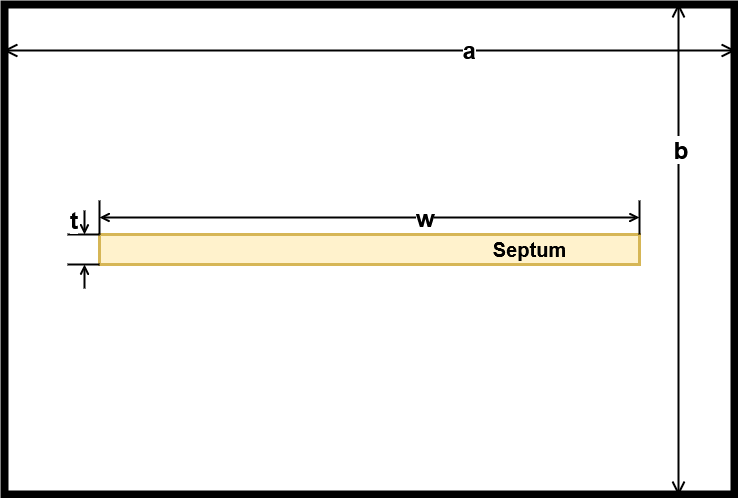
\includegraphics[width=0.5\linewidth]{content//10_theory//img/tem_cell_crosssection.png}
    \caption{Cross section of the TEM cell}
    \label{fig:tem_cell_crosssection}
\end{figure}

\begin{equation}
    f_c = \frac{c}{2} \sqrt{\left(\frac{m}{a}\right)^2 + \left(\frac{n}{b}\right)^2}
    \label{eqn:cutoff_frequency_rect_waveguide}
\end{equation}

\begin{itemize}
  \item \( f_c \): cutoff frequency of the mode \(\text{T}_{mn}\)
  \item \( c \): speed of light in the medium (approximately \(3 \times 10^8 \, \text{m/s}\) in air)
  \item \( a \): wider dimension (broad wall) of the rectangular waveguide (meters)
  \item \( b \): narrower dimension (narrow wall) of the rectangular waveguide (meters)
  \item \( m \): mode index in the \(a\)-direction (integer, \(m \geq 0\))
  \item \( n \): mode index in the \(b\)-direction (integer, \(n \geq 0\))
\end{itemize}

The cutoff frequency of the TE\textsubscript{10} mode is around 750\,MHz. To verify this, a modal analysis was performed in Ansys HFSS, where an empty TEM cell was modeled with two waveports defined at its output. The resulting S\textsubscript{12}-parameters are presented in\autoref{fig:te01_te10_tem_propagation}. The red line shows the S\textsubscript{12}-parameter over the frequency of the TEM mode, while the blue line demonstrates S\textsubscript{12}-parameter of the TE\textsubscript{10} mode. At a frequency of 750.2\,MHz, the mode propagates without attenuation, hence there is the cutoff frequency. The simulated result comes very close to the analytically determined one. The green line shows a cutoff frequency of 679.1\,MHz for the TE\textsubscript{01} mode. \autoref{eqn:cutoff_frequency_rect_waveguide} would predict a cutoff frequency of 1.5\,GHz, however, the septum influences n-odd modes like this one. Their cutoff frequencies are shifted to a lower value \cite{Weil_Gruner_1984}. 

%The first TM mode would be the TM\textsubscript{11} mode, since TM\textsubscript{01} and TM\textsubscript{10} do not exist.

In a real TEM cell, a tapered section transform the TEM waveguide to a coaxial transmission line. This section does not cause reflections of waves in TEM mode. However, higher order TE and TM modes get reflected, and because the TEM cell is a high-Q cavity, resonances occur at $\frac{\lambda}{4}$ or $\frac{\lambda}{2}$ \cite{990711}. This is not considered in these simulations, since the simulation model does not contain this tapered section. \todo{Maybe do simulations with such a tapered section. See \cite{990711}}

% \autoref{tab:even_n_modes} shows the cutoff frequencies of the n-even modes. The cutoff frequencies of the n-odd modes either have to be determined by the approximation in \cite{Wilson_Ma_1986} or analyzed numerically. \todo{Do either one of these}


% \begin{table}[h]
%     \centering
%     \begin{tabular}{ccc}
%         Mode & Calculated $f_c$ & Measured $f_c$\\
%         TE\textsubscript{10} & 750\,MHz & \\
%         TE\textsubscript{20} & 1.50\,GHz & \\
%         TE\textsubscript{12} & 3.09\,GHz & \\
%         TM\textsubscript{20} & 1.50\,GHz & \\
%         TM\textsubscript{12} & 3.09\,GHz & \\
%     \end{tabular}
%     \caption{Caption}
%     \label{tab:even_n_modes}
% \end{table}

\begin{figure}[h]
    \centering
    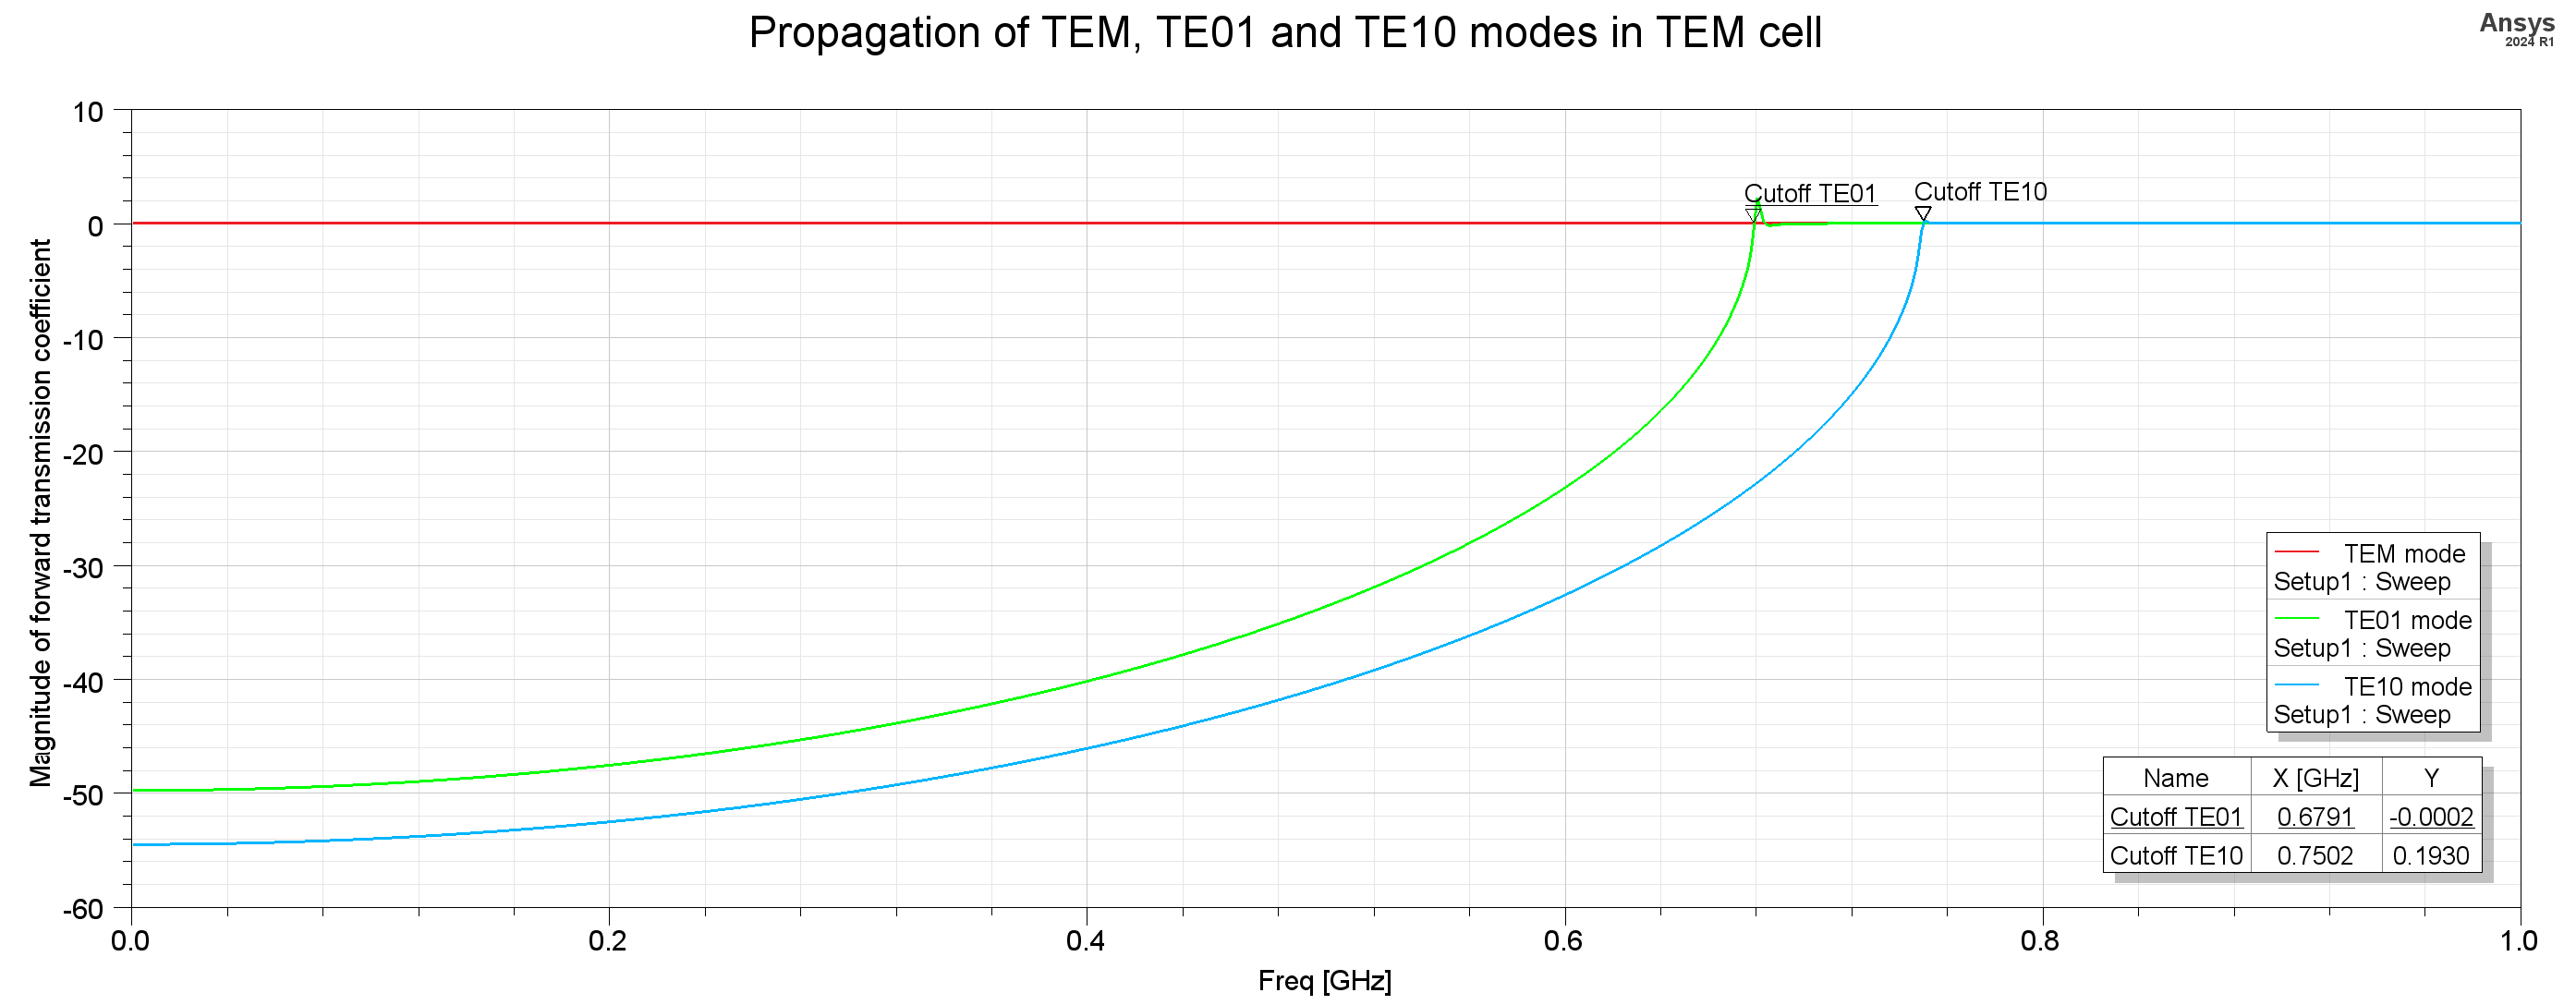
\includegraphics[width=1\linewidth]{content//10_theory//img/te01_te10_tem_propagation.png}
    \caption{Propagation of TEM, TE\textsubscript{01} and TE\textsubscript{10} modes in TEM cell}
    \label{fig:te01_te10_tem_propagation}
\end{figure}




The TEM cell does not only support TEM modes, above their cut-off frequency TE and TM modes begin to propagate. Because the TEM cell is a high-Q cavity, those cut-off frequencies are sharply defined frequencies. Due to imperfections, change in materials or finite conductivity of the conducting plates, wave propagating in the TEM mode may excite higher order TE and TM modes, too \cite{10791592}. A change in material, for example, demands the electric and magnetic field to have a component in the direction of propagation at the discontinuity. A paper by Wilson and Ma present analytical approximations to determine these frequencies \cite{Wilson_Ma_1986}.  There is a long list for the several first few corner frequencies of the first modes. Additionally, a paper by Koch, Groh and Garbe determines the resonance frequencies of the first TE modes analytically \cite{10791592}. The TEM mode is necessarily excited by the geometry of the TEM cell, hence this mode is called essential. The higher order TE and TM modes, which are only excited due to non-uniformity of the TEM cell, are called non-essential modes \cite{990711}.


The first modes propagating after the TEM mode is the TE\textsubscript{10} and TE\textsubscript{01} modes. Their transversal electric fields are depicted in \autoref{fig:transversal_e_fields_tem_cell}. 

\begin{figure}[h]
    \centering
    \begin{subfigure}[b]{0.3\linewidth}
        \centering
        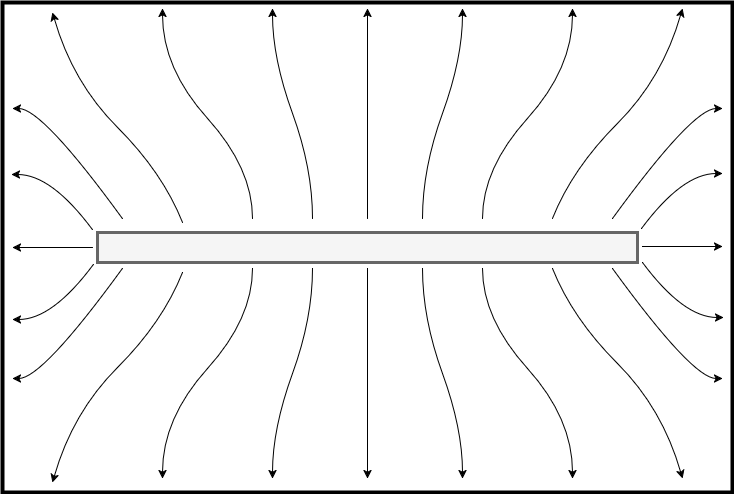
\includegraphics[width=\linewidth]{content/10_theory/img/tem_cell_mode.png}
        \caption{TEM Mode}
        \label{fig:tem_mode}
    \end{subfigure}
    \begin{subfigure}[b]{0.3\linewidth}
        \centering
        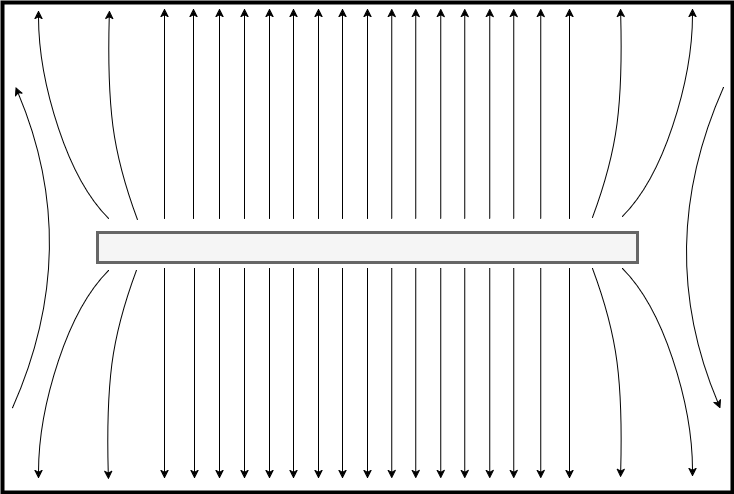
\includegraphics[width=\linewidth]{content/10_theory/img/te01_mode.png}
        \caption{TE\textsubscript{01}}
        \label{fig:te01_mode}
    \end{subfigure}
    \begin{subfigure}[b]{0.3\linewidth}
        \centering
        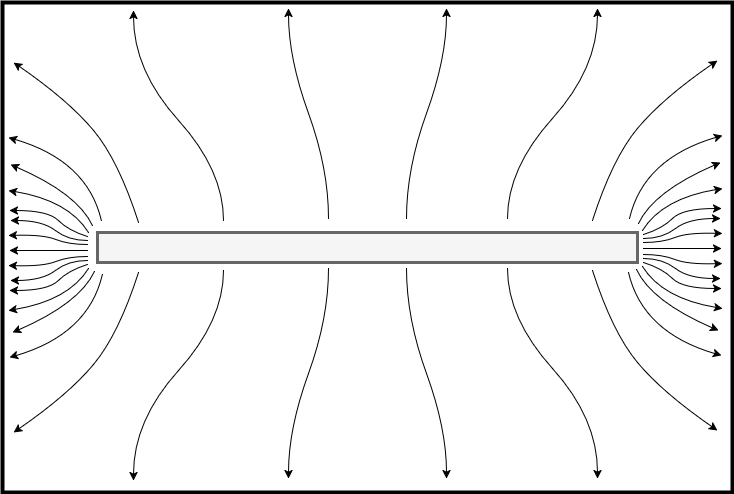
\includegraphics[width=\linewidth]{content/10_theory/img/te10_mode.png}
        \caption{TE\textsubscript{10}}
        \label{fig:te10_mode}
    \end{subfigure}
    \caption{Transversal electric fields in cross section of TEM cell}
    \label{fig:transversal_e_fields_tem_cell}
\end{figure}
\todo{Vector directions are wrong in the pictures. Additionally, update cutoff frequencies.}



